\claude{
\section[Measuring simplification from a scalar log]{Measuring simplification from a scalar log}\label{sec:method}
\subsection{Delay reconstruction}
\newcommand{\sgdstateexample}{%
In plain minibatch stochastic gradient descent (SGD), the optimizer state between updates is the parameter vector, $s_t=\theta_t$.
\ifdefined\newinmlcameraready
Given a sampled minibatch $B_t$ and a fixed learning rate $\eta$, the next iterate is $\theta_{t+1}=\theta_t-\eta\nabla_\theta L_{B_t}(\theta_t)$, where $L_{B_t}$ is the mean loss on that batch.
\fi
With momentum, $s_t=(\theta_t,m_t)$, where $m_t$ is an exponentially weighted sum of past minibatch gradients.
In either case, a weight-norm log records $x_t=\phi(s_t)=\|\theta_t\|_2$.}
\ifdefined\icompfinalcopy
We log a scalar $x_t=\phi(s_t)$ from state $s_t$.
\sgdstateexample{}
With fixed weights and no input, our recurrent generators have hidden state $s_t=\boldsymbol h_t$, dynamics $\boldsymbol h_{t+1}=F(\boldsymbol h_t)$, and activation $x_t=\tanh(h_{t,j})$ for neuron $j$.
\else
Suppose we have access only to a scalar log $x_1,\ldots,x_N$. At step $t$ we observe $x_t=\phi(s_t)$, where $s_t$ is the system state and $\phi$ is a scalar measurement function.
\ifdefined\newinmlcameraready
\sgdstateexample{}
\else
For example, in minibatch stochastic gradient descent (SGD) with fixed learning rate $\eta$, the state is the parameter vector $s_t=\theta_t$. Given a randomly sampled minibatch $B_t$, the next state is $\theta_{t+1}=\theta_t-\eta\nabla_\theta L_{B_t}(\theta_t)$, where $L_{B_t}$ is the mean loss on that batch. A weight-norm log records $x_t=\|\theta_t\|_2$. With momentum, the state also includes the velocity vector.
\fi
In our recurrent generators with fixed weights and no external input, the hidden state $s_t=\boldsymbol h_t$ evolves as $\boldsymbol h_{t+1}=F(\boldsymbol h_t)$. For neuron $j$ we record its activation $x_t=\tanh(h_{t,j})$, the value it passes to the rest of the network at step $t$.
\fi

\citet{takens1981detecting} gave conditions under which delay coordinates from a single scalar time series reconstruct \cx{the state space and dynamics of an autonomous system} up to a smooth change of coordinates. Related embedding theorems apply to systems with deterministic or stochastic forcing \citep{stark1999delay,stark2003delay}.

Within each sliding window, index its $W$ consecutive observations from 1 to $W$ and define $z_t=(x_t-\bar x)/\sigma_x$, where $\bar x$ and $\sigma_x>0$ are the window mean and standard deviation. For an integer lag $\tau\ge1$, the window yields $n=W-(E-1)\tau$ delay vectors with $E$ coordinates,
\begin{equation}
y_t=(z_t,z_{t+\tau},\ldots,z_{t+(E-1)\tau})\in\mathbb{R}^E,\qquad 1\le t\le n.
\label{eq:delay}
\end{equation}

\subsection{Pooled local-dimension estimation}\label{sec:mg-neighbors}
We take each delay vector $y_i$ in turn as the query point and search for neighbors within the same sliding window. When $\tau=1$, consecutive delay vectors share $E-1$ samples. Temporal correlations can persist even between disjoint segments. To limit their effect on the neighbor search, we use a Theiler window \citep{theiler1986spurious}. A candidate vector $y_\ell$ is an eligible neighbor of $y_i$ if their starting indices differ by more than $T$ samples, $|\ell-i|>T$. We rank these vectors by Euclidean distance $\|y_\ell-y_i\|_2$ in all $E$ coordinates (Figure~\ref{fig:method_geometry}). We retain the $k$ smallest distances $r_{i1}\le\cdots\le r_{ik}$, where $r_{ij}$ is the distance to the $j$th nearest eligible neighbor of $y_i$.

\begin{figure*}[!htbp]
\centering
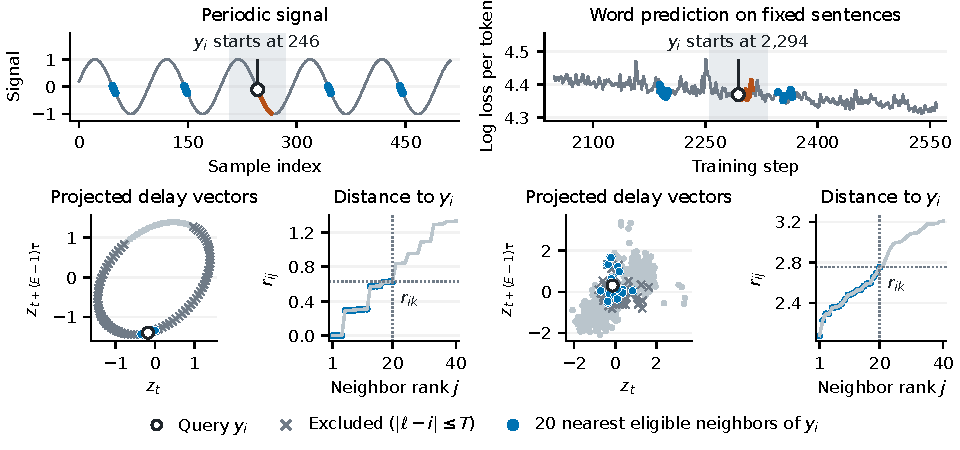
\includegraphics[width=\linewidth]{figures/icomp_method.pdf}
\caption{Once standardized, the orange samples give the coordinates of one point $y_i$ (open circle below). Blue dots on each series mark neighbor start indices outside the shaded Theiler window.}
\label{fig:method_geometry}
\end{figure*}

Suppose the delay vectors sample a smooth $d$-dimensional set with nearly constant density near $y_i$. The expected number of eligible vectors in a small ball of radius $r$ centered at $y_i$ then scales as $r^d$. Doubling the radius encloses about twice as many neighbors on a curve and four times as many on a surface. MG estimates this exponent by comparing the outer radius $r_{ik}$ with each of the $k-1$ inner distances and pooling the log ratios across all $n$ queries,
\begin{equation}
\MG=\frac{n(k-1)-1}
{\displaystyle\sum_{i=1}^{n}\sum_{j=1}^{k-1}
\log(r_{ik}/r_{ij})}.
\label{eq:mg}
\end{equation}
Under the local Poisson model, subtracting one in the numerator makes the estimate unbiased if the sums for different queries are independent (\appref{app:pooled-mg}). A lower estimate corresponds to slower growth of the neighbor count with radius. In figures and tables, the name after @ identifies the scalar time series used to form the delay vectors. For example, MG@loss denotes the MG of loss.

\subsection[Experimental questions]{Experimental questions}\label{sec:mg_conditions}
Consider the long-run fraction of time a trajectory spends within distance $r$ of a typical state. If this fraction scales as $r^d$ at small radii, $d$ is the local dimension of the distribution of visited states. When the delay map preserves distances up to constant factors, MG can estimate this exponent from repeated visits recorded in a scalar log (\appref{app:theory}). The reference dimension is one for a periodic orbit. For a waveform made from several tones, it equals the number of independent phases.

A training trajectory may pass through a region only once. We therefore ask whether a drop in MG coincides with a change we can measure independently, such as weight updates concentrating in fewer directions or a text encoder retaining less information about its input (Table~\ref{tab:experiment-questions}). For loss-spike warnings, we compare MG with log-loss roughness. Roughness is the standard deviation of successive log-loss differences divided by the standard deviation of log loss. We evaluate encoder selection by the resulting classification accuracy and forecaster selection by prediction error (Table~\ref{tab:decisions}).

\ifdefined\newinmlcameraready\else
\begin{table*}[!htbp]
\centering\small
\caption{What MG revealed from a single scalar log in selected experiments.}
\label{tab:experiment-questions}
\setlength{\tabcolsep}{4pt}
\begin{tabularx}{\linewidth}{@{}>{\raggedright\arraybackslash}p{.215\linewidth}>{\raggedright\arraybackslash}p{.19\linewidth}>{\raggedright\arraybackslash}X@{}}
\toprule
Experiment & Scalar log & Result \\
\midrule
\multicolumn{3}{@{}l}{\textbf{Can MG recover the number of independent phases?} (Section~\ref{sec:controlled} and \appref{app:controlled-observables})} \\
Sum of tones & Waveform amplitude & MG was close to one for four harmonics of a single frequency and close to four for four independent frequencies. \\
Diagonal matrix & Frobenius norm or one diagonal entry & As more entries oscillated independently, MG rose for the norm and stayed near one for a single oscillating entry. \\
Linear regression & Training loss & MG rose as more weight directions oscillated independently. \\
Recurrent tone generator & \cx{Single-neuron activation} & Among generators with four output peaks, MG increased with the number of independent phases. \\
Figure-eight generator & \cx{Single-neuron activation} & After training, MG was close to one and the full hidden state returned to nearly the same point each period. \\
\addlinespace
\multicolumn{3}{@{}l}{\textbf{How does MG compare with measurements of the weights or latent code?}} \\
Digit classifier (\appref{app:controlled-observables}) & Weight norm or gradient norm & On average, MG from the weight norm was closer to the effective dimension measured from weight covariance than MG from the gradient norm. \\
Small CIFAR-10 classifier (Section~\ref{sec:cnn}) & Weight norm & Training only the final layer reduced MG and concentrated updates in fewer directions. Keeping half the weights at zero reduced MG even as updates spread over more directions. \\
Text variational autoencoder (Section~\ref{sec:vae}) & Reconstruction loss on fixed sentences & Lower MG coincided with less mutual information between input sentences and their latent codes. \\
\addlinespace
\multicolumn{3}{@{}l}{\textbf{Can MG detect a training intervention or warn of a loss spike?} (Sections~\ref{sec:cnn} and \ref{sec:spike-warning})} \\
ResNet-18 & Weight norm & The rule fitted on the small classifier detected every run with a frozen feature extractor. It missed pruning and learning-rate reductions within the evaluation interval. \\
Transformer loss spikes & Logarithm of training loss & The MG rule detected 22 of 23 spikes in advance. The roughness rule detected all 23. Each produced 2.44 false alarms per 10,000 evaluated updates. \\
\addlinespace
\multicolumn{3}{@{}l}{\textbf{How well does MG select encoders or forecasters?} (Section~\ref{sec:ssl} and \appref{app:forecast_utility})} \\
Self-supervised MNIST encoders & Gradient norm & Linear classification accuracy for the encoder with the highest MG averaged 0.41 percentage points below the best in each repeat. \\
Activation forecasts & \cx{Single-neuron activation} & On held-out networks, choosing by MG or by validation gave similar mean forecast errors. \\
\bottomrule
\end{tabularx}
\end{table*}

\fi
}
